\documentclass[12pt]{article}

\usepackage[margin=2cm]{geometry}
\usepackage[T2A]{fontenc}
\usepackage[utf8]{inputenc}
\usepackage[russian]{babel}
\usepackage{multicol}
\usepackage{longtable}
\usepackage{graphics}
\usepackage{rotating}
\usepackage{float}

\setlength{\parindent}{0em}
\setlength{\parskip}{1em}

\usepackage{amsmath, amsfonts, amssymb, amsthm, mathtools}
\usepackage{icomma}

\title{Отчет о выполнении лабораторной работы \\ Определение вязкости воздуха по скорости течения через тонкие трубки}
\author{Лепарский Роман}
\date{\today}

\begin{document}

\maketitle

\newpage

\section{Аннотация}

\textbf{Цель работы:} экспериментально исследовать свойства течения газов по тонким трубкам при различных числах Рейнольдса; выявить область применимости закона Пуазейля и с его помощью определить коэффициент вязкости воздуха.

\section{Теоретические сведения}

 В данной работе нам предлагается исследовать течение газа через тонкие трубки. Характер этого течения определяется числом Рейнольдса:
 \begin{equation}
 	Re = \frac{\rho u a}{\eta}
 	\label{eq:reinolds}
 \end{equation}
 
 Экспериментально установлено, что в рамках данного опыта критическое число Рейнольдса $Re_{\text{кр}}$ ниже которого поток можно считать ламинарным равно $10^3$
 
 Найдем характерные для этого течения величины. 
 
 \begin{figure}[H]
 	\centering
 	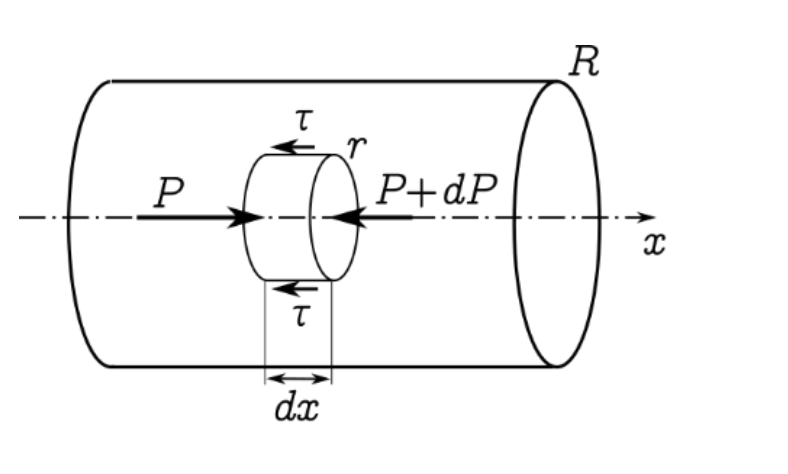
\includegraphics[scale = 0.3]{./images/puasel.png}
 	\label{fig:puasel}
 \end{figure}
 
 Для стационарного течения справедливо:
 
 \begin{align*}
 	F_{1x} &= -dP\cdot \pi r^2 \\
 	F_{2x} &= -\tau \cdot 2\pi r dx\\
 	\tau &= -\eta \frac{du}{dr}
 \end{align*}
 
 Из этих уравнений:
 \begin{equation}
	\frac{dp}{dx} = -\eta \frac{2}{r} \frac{du}{dr}
 \end{equation}
 
 Левая часть уравнения является градиентом давления, а правая не зависит от $x$. Поэтому справедливы следующие утверждения:
 
 \begin{align}
 	P(x) &= P_0 - \frac{\Delta P}{l}x \\
 	u(r) &= u_{max} - \frac{\Delta P}{4l}r^2
 \end{align}
 
 Если принять, что скорость газа вблизи стенок равна нулю, получим:
 \[
 	u(r) = \frac{\Delta P}{4l}(R^2 - r^2)
 \]
 
 Теперь можно получить формулу объемного расхода:
 \begin{equation}
 	Q = \int\limits_{0}^R u(r)\cdot 2\pi rdr = \frac{\pi R^4\Delta P}{8\eta l}
 	\label{eq:puasel}
 \end{equation}
 
 Формула Пуазейля (\ref{eq:puasel}) позволяет найти вязкость газа по зависимости расхода от перепада  давления в трубе и используется в качестве основной расчётной формулы в данной работе.
 
 Параболический профиль течения устанавливается не сразу, а только на некотором расстоянии $l_{\text{уст}} \approx 0,2R\cdot Re$
  \begin{figure}[H]
 	\centering
 	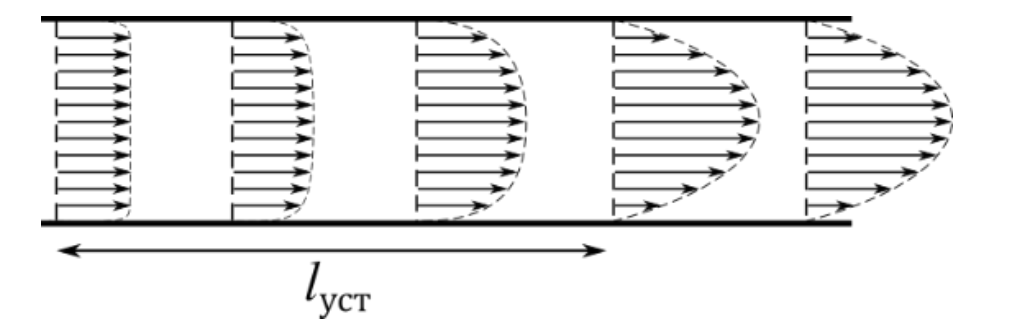
\includegraphics[scale = 0.2]{./images/lust.png}
 	\label{fig:lust}
 \end{figure}

Экспериментально длину установления можно определить, измеряя распределение давления вдоль трубки $P(x)$. На неустановившемся участке будет наблюдаться отклонение от линейного закона.

Коэффициент вязкости идеального газа можно описать следующей формулой:
\begin{equation}
	\eta \thicksim \frac{1}{3}\rho \bar{v}\lambda
\end{equation}

Для турбулентного течения в рамках некоторой теоретической модели можно получить соотношение 
\begin{equation}
	Q= \pi R^2 \bar{u} \thicksim R^{5/2} \sqrt{\frac{\Delta P}{\rho l}}
\end{equation}

\section{Экспериментальная установка}

\begin{figure}[H]
	\centering
	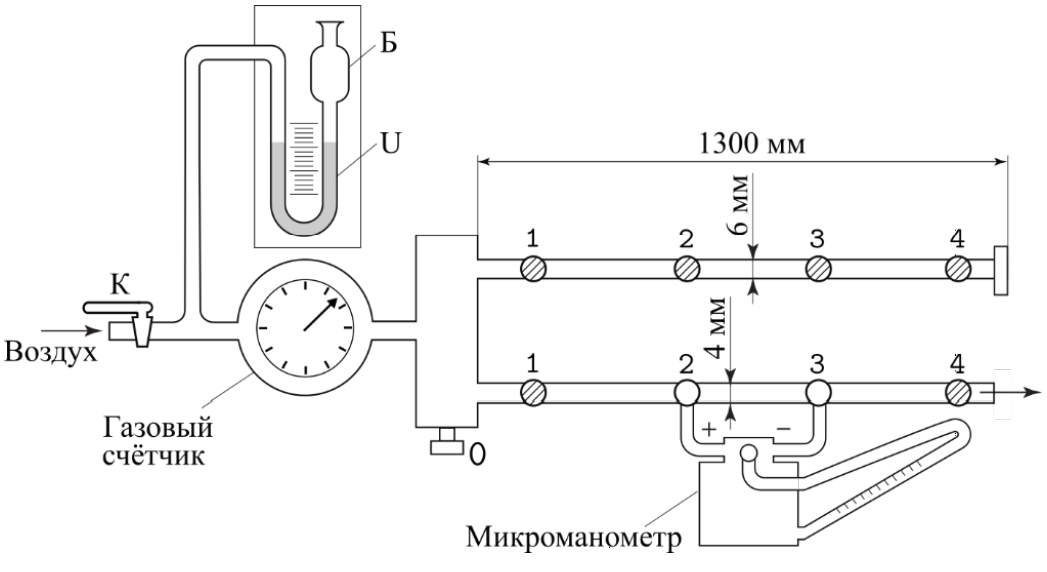
\includegraphics[scale = 0.4]{./images/stand.png}
	\caption{Схема установки}
	\label{fig:stand}
\end{figure}

Поток воздуха
под давлением, немного превышающим атмосферное, поступает через газовый счётчик в тонкие металлические трубки. Воздух нагнетается компрессором, интенсивность его подачи регулируется краном К. Трубки снабжены съёмными заглушками на концах и рядом миллиметровых отверстий, к которым можно подключать микроманометр. В рабочем состоянии открыта заглушка на одной (рабочей) трубке, микроманометр подключён к двум её выводам, а все остальные отверстия плотно закрыты пробками.

\section{Приборы и материалы}

В работе используются:

\begin{itemize}
	\item Система подачи воздуха;
	\item Газовый счетчик барабанного типа;
	\item Спиртовой микроманометр с регулируемым наклоном;
	\item Набор трубок различного диаметра с выходами для подсоединения микроманометра;
	\item Секундомер.
\end{itemize}

\section{Обработка результатов}



\section{Вывод}



\end{document}